\documentclass[12pt]{article}

% ---- Packages ----------------------------------------------------------------
\usepackage[margin=1in]{geometry}
\usepackage{booktabs}
\usepackage{graphicx}
\usepackage{amsmath}
\usepackage{natbib}
\usepackage{setspace}
\usepackage{hyperref}
\usepackage[font=small,labelfont=bf]{caption}

\doublespacing

% ---- Metadata ----------------------------------------------------------------
\title{Spatial Dynamics of Disappearances in Mexico, 2015--2024:\\
       A Municipal-Level Analysis by Outcome Status}

\author{[Author(s)]}
\date{\today}

% ==============================================================================
\begin{document}
\maketitle

% ---- Abstract ----------------------------------------------------------------
\begin{abstract}
[Abstract placeholder.]
\end{abstract}

\textbf{Keywords:} enforced disappearances; spatial autocorrelation; Mexico;
LISA; population bands; Norte; Baj\'io

% ---- 1. Introduction ---------------------------------------------------------
\section{Introduction}

[Introduction placeholder.]

% ---- 2. Data and Methods -----------------------------------------------------
\section{Data and Methods}

\subsection{Data}

[Data description placeholder.]

\subsection{Spatial Clustering Method}

We compute annual Local Moran's~$I$ (LISA) statistics for each of four RNPDNO
outcome statuses (Total, Not Located, Located Alive, Located Dead) using both
case counts and per-capita rates (per 100,000 inhabitants). Weights are based
on Queen contiguity; significance is assessed at $\alpha = 0.05$ using 999
conditional permutations. High-High (HH) clusters are defined as connected
components of statistically significant HH municipalities with a minimum size
of three municipalities.

% ---- 3. Results --------------------------------------------------------------
\section{Results}

\subsection{Regional Composition of HH Clusters, 2015 vs.\ 2024}

Table~\ref{tab:regional_shift} presents the regional distribution of
HH-cluster municipalities at the beginning and end of the study period.

\begin{table}[htbp]
\centering
\small
\caption{Regional Composition of High-High Disappearance Municipalities, 2015 vs 2024 (cases-based LISA, minimum cluster size = 3)}
\label{tab:regional_shift}
\resizebox{\textwidth}{!}{%
\begin{tabular}{lrrrrrrrrr}
\toprule
Region & \multicolumn{3}{c}{Not Located} & \multicolumn{3}{c}{Located Alive} & \multicolumn{3}{c}{Located Dead} \\
\cmidrule(lr){2-4}\cmidrule(lr){5-7}\cmidrule(lr){8-10}
 & 2015 & 2024 & $\Delta$ & 2015 & 2024 & $\Delta$ & 2015 & 2024 & $\Delta$ \\
\midrule
Norte & 20 & 15 & -5 & 4 & 15 & +11 & 0 & 21 & +21 \\
Norte--Occidente & 0 & 6 & +6 & 0 & 0 & +0 & 0 & 5 & +5 \\
Centro--Norte & 10 & 0 & -10 & 4 & 3 & -1 & 0 & 4 & +4 \\
Centro & 14 & 43 & +29 & 48 & 45 & -3 & 22 & 40 & +18 \\
Sur & 0 & 5 & +5 & 3 & 0 & -3 & 0 & 0 & +0 \\
\midrule
\quad \textit{of which Bajío} & 10 (42\%) & 10 (23\%) & +0 & 32 (62\%) & 3 (6\%) & -29 & 13 (59\%) & 9 (20\%) & -4 \\
\midrule
$\chi^2$ \textit{p}-value & \multicolumn{3}{c}{$p < 0.001$} & \multicolumn{3}{c}{$p = 0.023$*} & \multicolumn{3}{c}{$p = 0.003$**} \\
\bottomrule
\end{tabular}}
\par\vspace{4pt}
\begin{minipage}{\textwidth}\footnotesize\textit{Note}: Counts are municipalities in High-High spatial clusters ($\alpha = 0.05$, 999 permutations, Queen contiguity, min.\ size = 3). ``of which Baj\'io'' = HH municipalities flagged as Baj\'io, as \% of Centro-Norte + Centro HH municipalities. $\chi^2$ tests that regional composition is identical in 2015 and 2024 (zero-sum columns excluded).\end{minipage}
\end{table}

\subsection{Trend Slopes by Geography and Status}

Table~\ref{tab:trend_slopes} reports OLS trend slopes (municipalities per year)
for Norte and Baj\'io under each status--metric combination.

\begin{table}[htbp]
\centering
\small
\caption{Linear Trend Slopes (Municipalities per Year) in High-High Clusters, Norte vs Bajío, by Outcome Status and Metric (2015--2024)}
\label{tab:trend_slopes}
\begin{tabular}{llrrrr}
\toprule
 & & \multicolumn{4}{c}{Outcome status} \\
\cmidrule(lr){3-6}
Geography & Metric & Total & Not Located & Located Alive & Located Dead \\
\midrule
Norte & Cases & +1.03 & -0.56 & +1.42** & +2.29*** \\
 & Rates & +1.49 & -0.64 & +2.25 & +0.78 \\
\midrule
Bajío & Cases & -2.12* & +0.21 & -2.19* & +0.17 \\
 & Rates & -0.51 & +0.41 & -2.10 & +1.18 \\
\bottomrule
\end{tabular}
\par\vspace{4pt}
\begin{minipage}{\textwidth}\footnotesize\textit{Note}: OLS slope = municipalities/year. $^{*}p<0.05$, $^{**}p<0.01$, $^{***}p<0.001$. Baj\'io row includes HH cluster municipalities where $\geq$50\% of cluster members are Baj\'io-flagged; Norte excludes Baj\'io-flagged municipalities.\end{minipage}
\end{table}

\subsection{Temporal Trends in HH Cluster Size}

Figure~\ref{fig:hh_trend} plots the annual number of municipalities in HH
clusters for Norte and Baj\'io across all four outcome statuses.

\begin{figure}[htbp]
  \centering
  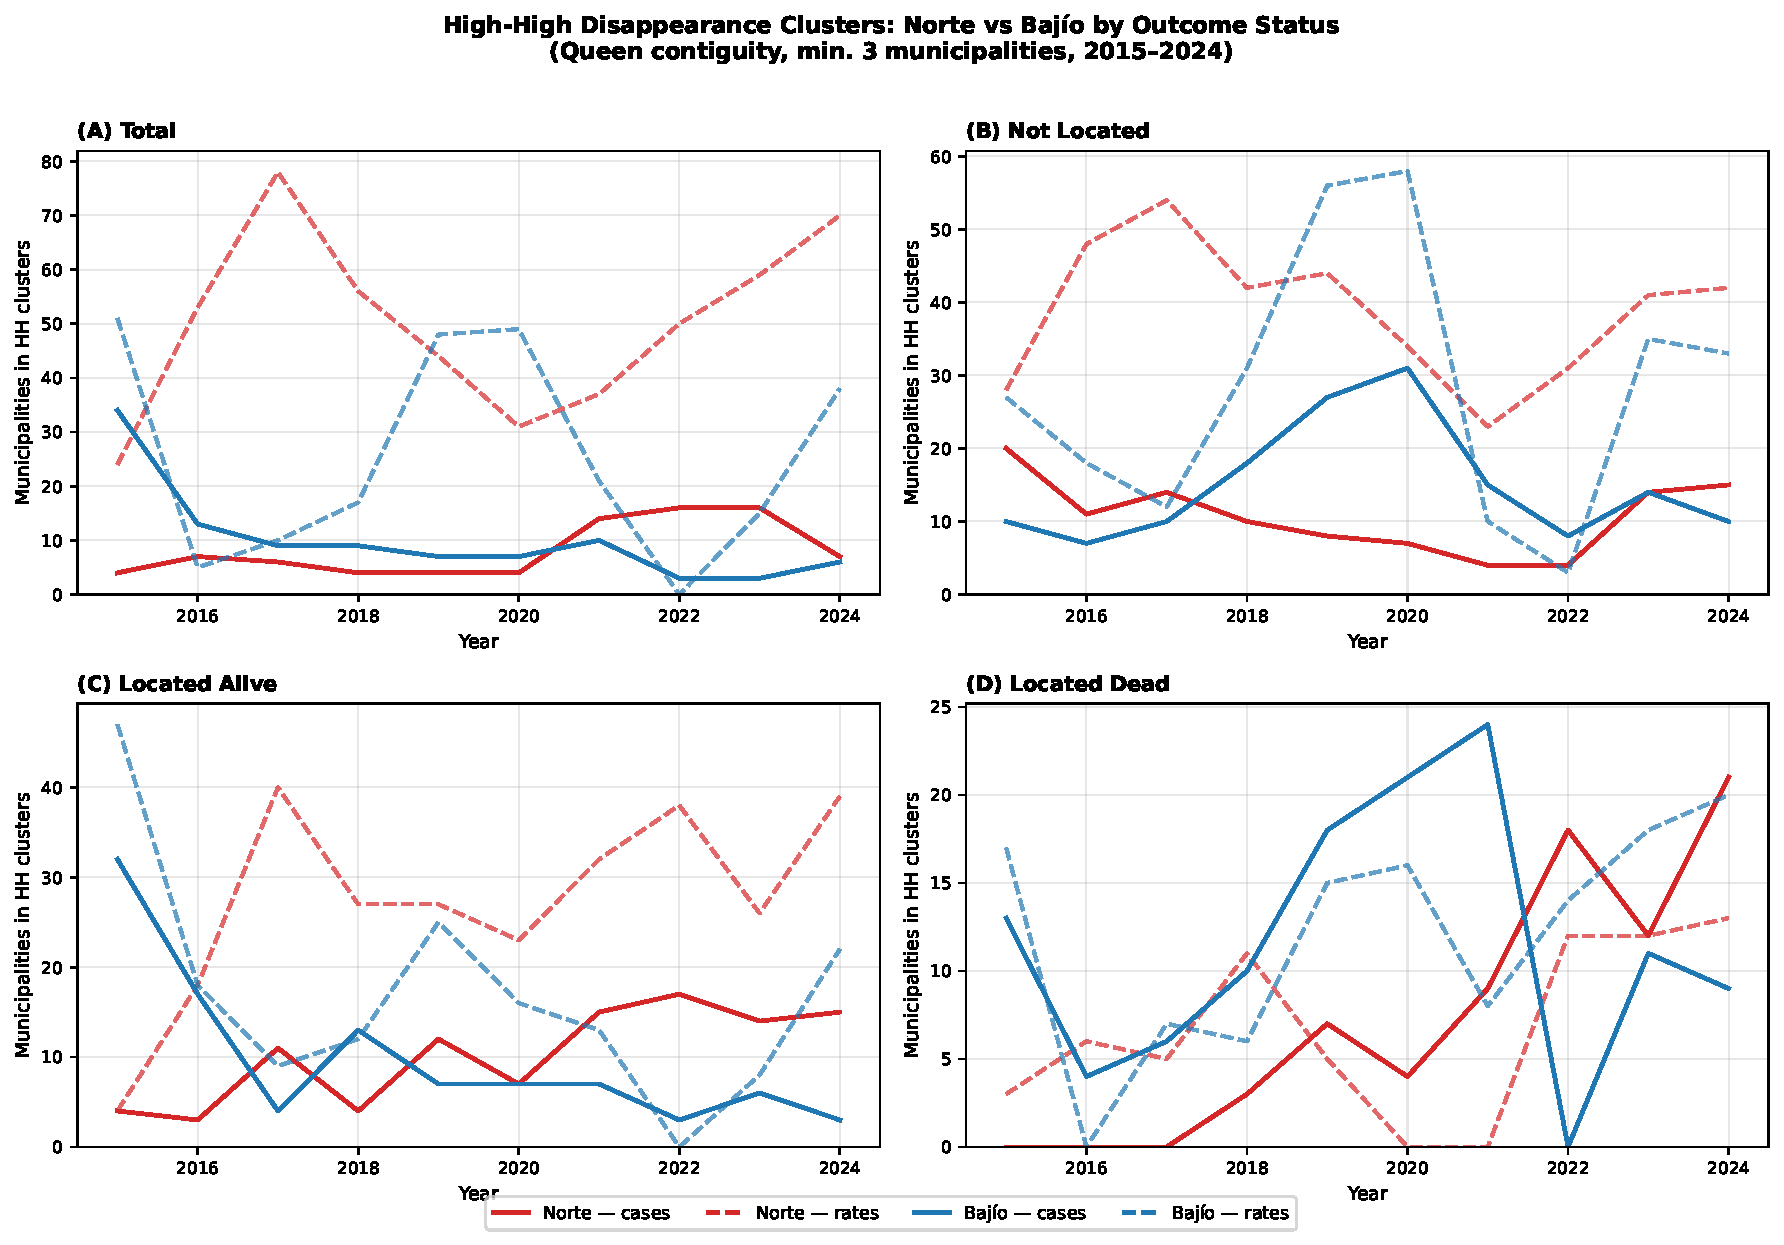
\includegraphics[width=\textwidth]{figures/fig1_hh_trend_by_status.pdf}
  \caption{High-High disappearance cluster municipalities in Norte and Baj\'io
           by outcome status, 2015--2024. Solid lines = case-based LISA;
           dashed lines = rate-based LISA.}
  \label{fig:hh_trend}
\end{figure}

\subsection{Divergence Between Case-Based and Rate-Based Hotspots}

Figure~\ref{fig:jaccard} shows annual Jaccard similarity between case-based
and rate-based HH municipality sets.

\begin{figure}[htbp]
  \centering
  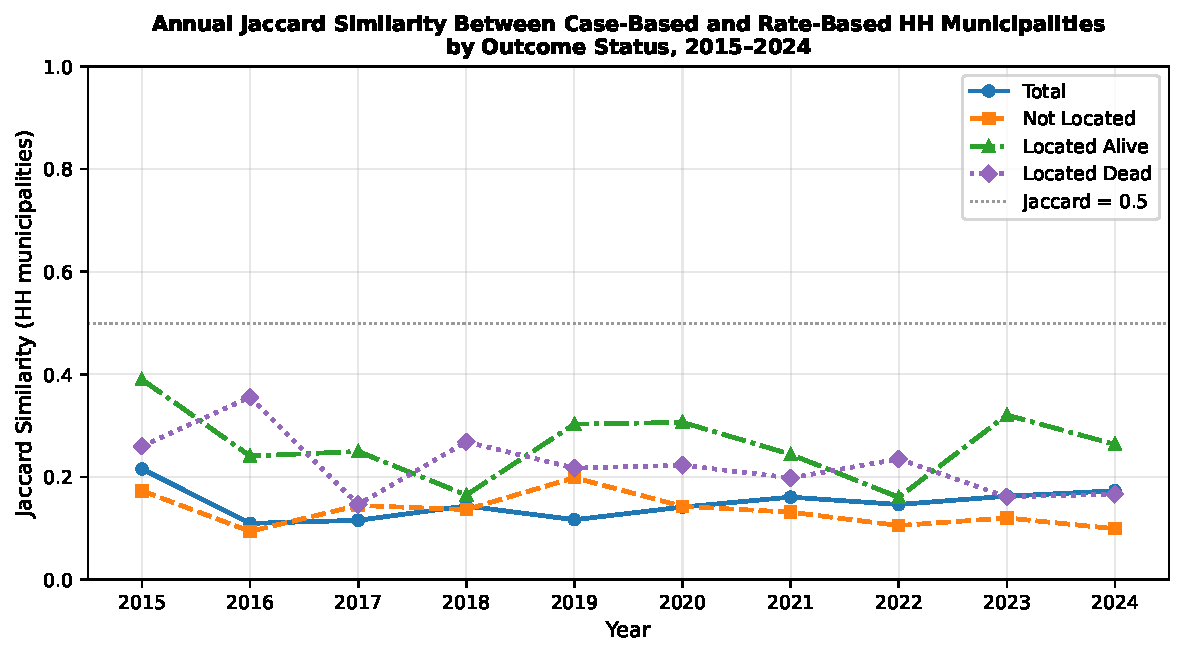
\includegraphics[width=0.8\textwidth]{figures/fig2_cases_vs_rates_jaccard.pdf}
  \caption{Annual Jaccard similarity between case-based and rate-based
           HH municipalities by outcome status, 2015--2024.}
  \label{fig:jaccard}
\end{figure}

\subsection{Spatial Distribution, 2015 vs.\ 2024}

Figure~\ref{fig:maps} maps HH municipalities for Located Alive and Located Dead
at the start and end of the study period.

\begin{figure}[htbp]
  \centering
  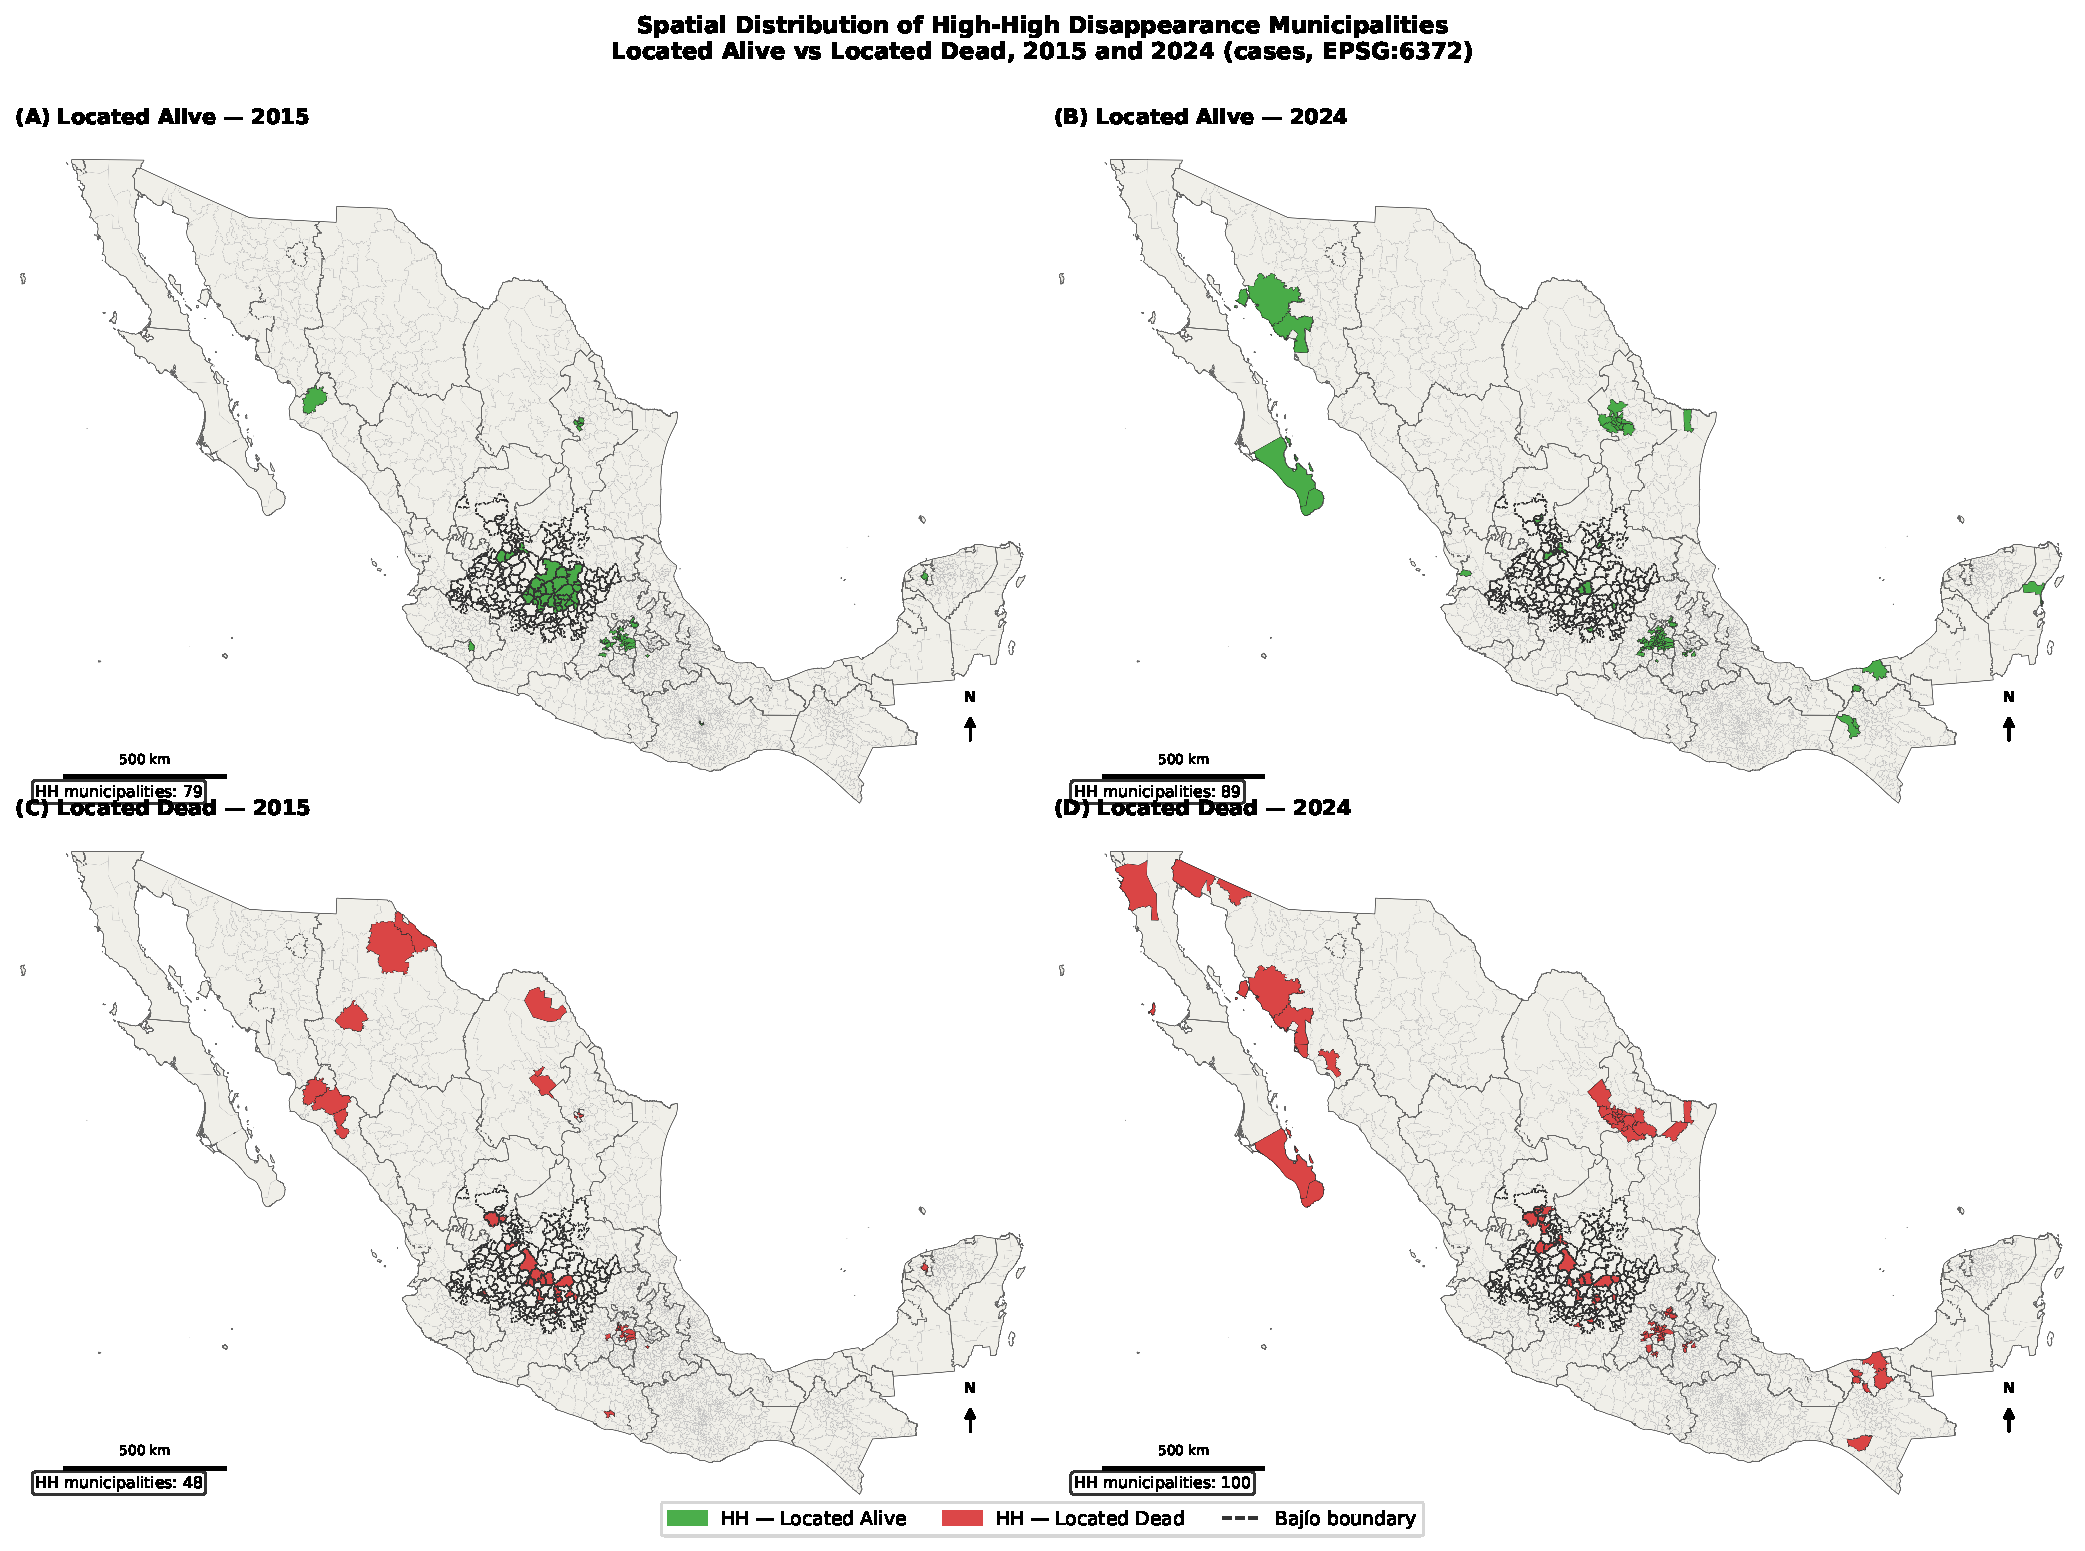
\includegraphics[width=\textwidth]{figures/fig3_hh_maps_2015_2024.pdf}
  \caption{Spatial distribution of High-High disappearance municipalities
           for Located Alive (green) and Located Dead (red), 2015 and 2024.
           Dashed border: Baj\'io region. Projection: EPSG:6372.}
  \label{fig:maps}
\end{figure}

% ---- 4. Discussion -----------------------------------------------------------
\section{Discussion}

[Discussion placeholder.]

% ---- 5. Conclusion -----------------------------------------------------------
\section{Conclusion}

[Conclusion placeholder.]

% ---- References --------------------------------------------------------------
\bibliographystyle{apalike}
\bibliography{references}

\end{document}
